% Migrated from the user-supplied IJACSA 2026 Paper_format.tex.
% The supplied IEEEtran.cls is used without modifications.
% Original template: bare_conf.tex, Michael Shell; LPPL notices retained
% in SAI_Paper_Format_Latex/Paper_format.tex and IEEEtran.cls.
\documentclass[conference,letterpaper]{IEEEtran}
\usepackage[T1]{fontenc}
\usepackage[utf8]{inputenc}
\usepackage[english]{babel}
\usepackage[cmex10]{amsmath}
\usepackage{array,amssymb,amsfonts,color,float}
\usepackage{graphicx,adjustbox}
\usepackage{fancyhdr}
\usepackage{subcaption}
\usepackage{flushend}
\captionsetup[table]{justification=centering,labelsep=period,font={footnotesize,sc}}
\captionsetup[figure]{justification=centering,labelsep=period,font={footnotesize}}
\usepackage{booktabs,threeparttable}
\usepackage{algorithm,algpseudocode}
\usepackage{tikz,pgfplots,fontawesome5}
\usetikzlibrary{arrows.meta,positioning,babel}
\pgfplotsset{compat=1.18}
\usepackage{xurl}
\usepackage[hidelinks]{hyperref}
\urlstyle{same}
\floatname{algorithm}{Algorithm}
\algrenewcommand{\algorithmicrequire}{\textbf{Input:}}
\algrenewcommand{\algorithmicensure}{\textbf{Output:}}
\newcommand{\Pos}{\mathrm{Pos}}
\newcommand{\Neg}{\mathrm{Neg}}
\newcommand{\Neu}{\mathrm{Neu}}
\pagestyle{fancy}
\fancyhf{}
\setlength{\headheight}{24pt}
\setlength{\footskip}{20pt}
\fancyhead[R]{\textit{(IJACSA) International Journal of Advanced Computer Science and Applications, \\
Vol. XXX, No. XXX, 2026}}
\renewcommand{\headrulewidth}{0pt}
\fancyfoot[C]{www.ijacsa.thesai.org}
\renewcommand{\footrulewidth}{0.5pt}
\fancyfoot[R]{\thepage\ $|$ P a g e}
\setcounter{page}{1}
\begin{document}


%
% paper title
% can use linebreaks \\ within to get better formatting as desired
\title{Expressed Affective Polarization in YouTube Comments During the 2026 Peruvian Presidential Election}


% author names and affiliations
% use a multiple column layout for up to three different
% affiliations
\makeatletter
\newcommand{\linebreakand}{
  \end{@IEEEauthorhalign}
  \hfill\mbox{}\par
  \mbox{}\hfill\begin{@IEEEauthorhalign}
}
\makeatother
\author{
\IEEEauthorblockN{Jose Alva Cornejo, Roxana Flores-Quispe, Yuber Velazco-Paredes}
\IEEEauthorblockA{Universidad Nacional de San Agustín de Arequipa, Arequipa, Perú}
%Emails: jalvac@unsa.edu.pe, rfloresqu@unsa.edu.pe, yvelazco@unsa.edu.pe
}




% conference papers do not typically use \thanks and this command
% is locked out in conference mode. If really needed, such as for
% the acknowledgment of grants, issue a \IEEEoverridecommandlockouts
% after \documentclass

% for over three affiliations, or if they all won't fit within the width
% of the page, use this alternative format:
% 
%\author{\IEEEauthorblockN{Michael Shell\IEEEauthorrefmark{1},
%Homer Simpson\IEEEauthorrefmark{2},
%James Kirk\IEEEauthorrefmark{3}, 
%Montgomery Scott\IEEEauthorrefmark{3} and
%Eldon Tyrell\IEEEauthorrefmark{4}}
%\IEEEauthorblockA{\IEEEauthorrefmark{1}School of Electrical and Computer Engineering\\
%Georgia Institute of Technology,
%Atlanta, Georgia 30332--0250\\ Email: see http://www.michaelshell.org/contact.html}
%\IEEEauthorblockA{\IEEEauthorrefmark{2}Twentieth Century Fox, Springfield, USA\\
%Email: homer@thesimpsons.com}
%\IEEEauthorblockA{\IEEEauthorrefmark{3}Starfleet Academy, San Francisco, California 96678-2391\\
%Telephone: (800) 555--1212, Fax: (888) 555--1212}
%\IEEEauthorblockA{\IEEEauthorrefmark{4}Tyrell Inc., 123 Replicant Street, Los Angeles, California 90210--4321}}




% use for special paper notices
%\IEEEspecialpapernotice{(Invited Paper)}


% make the title area
\maketitle
\thispagestyle{fancy}


\begin{abstract}
Electoral campaigns provided opportunities to observe how support for a political option coexisted with rejection of its opponents, but general comment sentiment did not identify the recipient of an evaluation. This study examined expressed affective polarization on YouTube during the 2026 Peruvian presidential election through explicit evaluations of political actors. Observed political affinity was identified in one partition of videos, while evaluations across blocs were compared in another, separating the evaluated target from the channel's editorial orientation. Among 122 users with sufficient evidence toward both blocs, the mean normalized gap was 1.44 (95\% CI [1.27, 1.68]). The positive contrast persisted across changes in event support, video contributions, and the presence of frequently mentioned actors. A complementary comparison of five classifiers distinguished target identification from sentiment classification in the evaluation of automated measurement. The findings documented a consistent pattern of expressed affective polarization among the studied users: support for aligned political actors coexisted with rejection of opponents, including in discussions hosted by neutral news sources. The study contributed a reproducible approach to identifying how political alignment was expressed through evaluations of rival actors in Peru's electoral discussion.

\end{abstract}

% IEEEtran.cls defaults to using nonbold math in the Abstract.
% This preserves the distinction between vectors and scalars. However,
% if the conference you are submitting to favors bold math in the abstract,
% then you can use LaTeX's standard command \boldmath at the very start
% of the abstract to achieve this. Many IEEE journals/conferences frown on
% math in the abstract anyway.

% no keywords


\begin{IEEEkeywords}
Sentiment analysis; Natural language processing; Social computing; Targeted sentiment analysis; Affective polarization; Social media; Transformer models; YouTube; Peruvian elections.
\end{IEEEkeywords}


% For peer review papers, you can put extra information on the cover
% page as needed:
% \ifCLASSOPTIONpeerreview
% \begin{center} \bfseries EDICS Category: 3-BBND \end{center}
% \fi
%
% For peerreview papers, this IEEEtran command inserts a page break and
% creates the second title. It will be ignored for other modes.
\IEEEpeerreviewmaketitle



\section{Introduction}

Social media had become prominent spaces for political discussion and the expression of citizens' opinions. 
Platforms such as Facebook, Twitter/X, and YouTube hosted posts, comments, and exchanges about candidates, 
parties, and public policy \cite{statista2026}. These records provided material for studying political 
communication with natural language processing (NLP) \cite{ref1}. Engagement with political content had also 
been associated with more polarized opinions: Afyare \cite{afyare2025socialmedia} described platforms as spaces 
for both mobilization and confrontation. Analyzing public comments could therefore reveal how political options 
were discussed, while the people who commented remained distinct from the population of voters.

Sentiment analysis usually classified the polarity of a text as positive, negative, or neutral. Advances in 
deep learning and Transformer models had improved contextual text classification \cite{Singh2026}. These 
methods had also informed computational research on affective polarization. Martínez-España et al. \cite{polariz} proposed an individual measure derived from social media posts; Bor et al. \cite{bor2023} examined sentiment across political groups and policy issues. In Peru, earlier elections and political discussions had been studied using both conventional representations and deep models \cite{Ayma2024,Carrera2026}. Ponte Torrel \cite{Ponte2022} examined affective expressions during the 2021 presidential runoff, while Mejía Navarrete \cite{Mejia2024} analyzed political polarization over 2000--2023.

The 2026 election provided a relevant setting for studying these expressions. The first presidential round took place on April 12, followed by a June 7 runoff between Fuerza Popular and Juntos por el Perú, as documented by the national electoral authority \cite{JNE11352026}. The Defensoría del Pueblo recorded disputes over the electoral process and opposition to political candidacies during this period \cite{Defensoria2842026}. These records established the context in which the comments were produced; they did not show that the same disputes caused any pattern measured here. The study's January--June window covered multiple stages of the contest, rather than a single electoral event.

Two methodological issues motivated the study. First, access restrictions on platforms such as Twitter/X encouraged research on other discussion environments \cite{ANTONAKAKI2021114006}, including YouTube's channel--video--comment structure. Second, general language models could struggle with informal Spanish, local political slang, sarcasm, and dialectal variation \cite{10.1145/3446132.3446424,robertuito}. Interpretation also required identifying the recipient of an evaluation: a negative comment under a neutral news source could reject an actor from either political bloc. The source's editorial orientation could not simply be assigned to the author or the actor being discussed.

This work developed a reproducible observational study of targeted political sentiment and expressed affective polarization using 1\,012\,515 public YouTube comments from January--June 2026. The study examined 300 user histories in a fixed order; 122 contained sufficient evaluable evidence toward both political blocs. The analysis calculated AP, $\mathrm{AP}_{In}$, $\mathrm{AP}_{Out}$, and dispersion (\textit{spread}), and used a normalized gap with uncertainty intervals as the primary contrast.

The method adapted the formulation of Martínez-España et al. \cite{polariz} to YouTube. It evaluated explicit mentions of political actors, retained editorial orientation as source information, and separated the videos used to identify observed political affinity from those used to measure evaluations. Neutral sources remained in the observation frame without becoming a third target bloc or an experimental control. User-level measurement was examined separately from Transformer classification: the availability of a large comment collection did not establish that every comment could be classified reliably. The resulting contribution concerned the direction, robustness, and limits of political evaluations expressed by the observed users.

Section II reviewed related work. Section III described data acquisition, preprocessing, targeted classification, and the measurement definitions. Section IV presented results and their interpretation. Sections V and VI discussed limitations and conclusions, respectively.

\section{Related Work}
Political sentiment analysis had gained attention as user-generated social media content increased and advanced NLP techniques became available. Recent research had approached this problem through the study of political polarization, automated opinion classification, and models specialized in informal language.

One research strand examined political polarization through sentiment analysis. Martínez-España et al. \cite{polariz} proposed a methodology for measuring individual affective polarization using Transformer models applied to social media data. Their work provided a computational precedent for studying affective expressions; text-based measurements and surveys did not constitute equivalent instruments. Similarly, Bor et al. \cite{bor2023} used sentiment analysis to quantify political polarization on Twitter across political groups and public policy issues in the United States, finding significant differences in polarization levels by topic.

Another strand focused on automated political sentiment classification using machine learning and deep learning. In Peru, Ayma et al. \cite{Ayma2024} analyzed Twitter/X posts from the 2021 presidential election using TF-IDF and Word2Vec representations with conventional classifiers, obtaining F1 scores above 0.93. Carrera et al. \cite{Carrera2026} subsequently compared conventional text representations and Transformer models for classifying comments about Peruvian legislative proposals. Their results showed that Transformers consistently outperformed conventional approaches, with reported accuracy above 88\%.

Pandey et al. \cite{pandey2025twitter} analyzed voter sentiment during the 2025 Bihar legislative election using more than 1\,100 posts collected through the Twitter API. The authors compared Random Forest, Support Vector Machine (SVM), and BERT sentiment classifiers. Posts were initially labeled using VADER, and party-level trends were then evaluated with the \textit{Net Sentiment Score} (NSS). BERT achieved 80\% accuracy and outperformed the conventional models, illustrating the use of Transformers for electoral sentiment analysis with a small dataset.

% Chire Saire y Vilca Zuñiga \cite{chire2021analysis} analizaron la reacción de los usuarios de Twitter ante el proceso de vacancia presidencial ocurrido en Perú durante la pandemia por COVID-19. El estudio tuvo como objetivo identificar los principales temas de discusión y evaluar el impacto que la crisis política generó en la población peruana a partir de las publicaciones realizadas en esta red social. Los autores recopilaron mensajes relacionados con el proceso de destitución presidencial y realizaron un análisis de las opiniones expresadas por los usuarios para identificar tendencias en el debate político. Los resultados evidenciaron que Twitter constituyó una fuente relevante para analizar la percepción ciudadana y la reacción de la población frente a los acontecimientos políticos ocurridos durante dicho periodo.

Rizk et al. \cite{rizk2023predicting} proposed a model for predicting the 2020 United States presidential election using geolocated Twitter posts. Their methodology combined sentiment analysis, a Multinomial Naive Bayes classifier, and machine learning to estimate the popular vote and electoral votes across all 50 states. The authors also removed bot-generated posts and outliers, examined temporal and spatial changes in public opinion, and used network analysis and community detection to identify user interaction patterns. Their model correctly predicted Joe Biden's victory and achieved 89.9\% agreement with the official election results.

Rodríguez-Ibáñez et al. \cite{rodriguez2021sentiment} studied sentiment in Twitter posts related to the 2019 Spanish election. They collected thousands of posts before and after the election and proposed a two-stage methodology: statistical characterization using entropy, mutual information, and the \textit{Compounded Aggregated Positivity Index} (CAPI), followed by feature extraction through nonlinear learning, including autoencoders and stochastic embedding methods. Both the statistical metrics and learned representations characterized temporal changes in sentiment and differences in polarity across political parties and leaders during the electoral period.

Chaudhry et al. \cite{chaudhry2022sentiment} analyzed Twitter sentiment before, during, and after the 2020 United States presidential election. They collected posts through the Twitter API, applied preprocessing and TF-IDF feature extraction, and used a Naive Bayes classifier to determine polarity. The authors compared their findings with official election results and examined swing states and states considered atypical. Expressed sentiment agreed with electoral outcomes in most cases and varied across the periods studied. The classifier achieved 94.58\% accuracy and 93.19\% precision.

More recent studies examined polarization and sentiment specifically on YouTube. Miehling et al. \cite{Miehling2025} analyzed more than three million comments from news channels during the Israel--Hamas conflict using aspect-based sentiment analysis. Their findings showed that a comment's general sentiment did not necessarily reflect the author's stance toward a specific political entity. This distinction motivated the separation between general sentiment and comment--target evaluations adopted in this study.

Together, these studies demonstrated the usefulness of Transformer models for analyzing political discourse and sentiment. They also motivated extending these methods to audiovisual platforms such as YouTube, distinguishing editorial provenance from political targets, and adapting representations to regional slang and dialectal variation.

\section{Proposed Method}

\begin{figure*}[t]
\centering
\resizebox{0.95\textwidth}{!}{\begin{tikzpicture}[x=1cm,y=1cm,>=Latex,
 box/.style={draw=black!25,rounded corners=2mm,fill=black!2,
   text width=4.6cm,minimum height=1.55cm,align=center,
   execute at begin node={\hyphenpenalty=10000\exhyphenpenalty=10000},font=\sffamily\small,inner sep=3mm},
 leftbox/.style={box,text width=6cm,draw=blue!50!black,fill=blue!3},
 rightbox/.style={box,text width=6cm,draw=teal!65!black,fill=teal!3},
 flow/.style={->,line width=.8pt,draw=black!65},
 lab/.style={font=\sffamily\small,fill=white,inner sep=2pt}]
\node[box] (api) at (2.5,0) {
\includegraphics[height=6mm]{docs/figures/youtube_icon.pdf}\\
  \textbf{Data extraction}\\YouTube Data API · comments and replies};
\node[box] (prep) at (8.5,0) {{\Large\faFilter}\\
  \textbf{Preparation}\\Dates, provenance, and deduplication};
\node[box] (corpus) at (14.5,0) {{\Large\faDatabase}\\
  \textbf{Comment collection}\\Frozen study data};
\draw[flow] (api)--(prep); \draw[flow] (prep)--(corpus);
\node[leftbox] (users) at (4.2,-2.6) {{\Large\faUsers}\\
  \textbf{Histories of 300 users}\\First users in the fixed order; all their comments};
\node[rightbox] (benchmark) at (12.8,-2.6) {{\Large\faClipboardList}\\
  \textbf{Evaluation sample}\\3,000 comments; annotated targets and evaluations};
\draw[flow] (corpus.south)--++(0,-.3)-|(users.north);
\draw[flow] (corpus.south)--++(0,-.3)-|(benchmark.north);
\node[leftbox] (targets) at (4.2,-4.9) {{\Large\faTags}\\
  \textbf{Comment--target evaluation}\\Explicit mentions and events by political bloc};
\node[rightbox] (train) at (12.8,-4.9) {{\Large\faMicrochip}\\
  \textbf{Training · Kaggle GPU}\\Three references and two additional models\\Three seeds per model};
\draw[flow] (users)--(targets);
\node[leftbox] (ab) at (4.2,-7.2) {{\Large\faProjectDiagram}\\
  \textbf{A/B video split}\\A: observed political affinity\\B: affective comparison};
\node[rightbox] (eval) at (12.8,-7.2) {{\Large\faBalanceScale}\\
  \textbf{Classifier evaluation}\\End-to-end extraction and common context};
\draw[flow] (targets)--(ab);
\draw[flow] (train)--node[lab,right]{Predictions}(eval);
\draw[flow] (benchmark.east)--++(.65,0)|-node[lab,pos=.65,right]{Reference}(eval.east);
\node[leftbox] (measure) at (4.2,-10.7) {{\Large\faChartBar}\\
  \textbf{Observational measurement}\\AP\textsubscript{In}, AP\textsubscript{Out}, AP, dispersion\\Normalized gap, intervals, and support\\Sensitivity and individual stability};
\node[rightbox] (models) at (12.8,-10.7) {{\Large\faChartLine}\\
  \textbf{Model comparison}\\Per-class F1, coverage, and errors};
\draw[flow] (ab)--(measure); \draw[flow] (eval)--(models);
\end{tikzpicture}
}
\caption{Study workflow. The left branch measured affective expressions in user histories and examined event support, sensitivity, and individual stability. The right branch evaluated classifiers using separate development data. User-history measurement did not depend on classifier training or predictions.}
\label{fig:metodo}
\end{figure*}

Figure~\ref{fig:metodo} summarized acquisition through YouTube Data API v3, preprocessing with editorial provenance, separate user-history and evaluation samples, and metric computation. User-level measurement and classifier evaluation had different inputs and denominators. Affective polarization was operationalized as differential evaluation of political actors across blocs; reply counts and survey-based ideological distance were separate constructs.

\subsection{Data acquisition}

YouTube was selected as the primary data source given access restrictions on other platforms \cite{ANTONAKAKI2021114006}. Its official API organized observations into channels and videos, allowing comments to retain traceable editorial provenance.

Editorial groups were documented using external sources on media ownership, party affiliation, and editorial orientation. The observed union contained 40 channels: ten right-wing, eight left-wing, and 22 neutral sources. This included historical records and the expanded capture and did not imply balanced source representation. The \textit{party} field identified source provenance only, not the author's affiliation or the target's bloc. Neutral sources were not an experimental control.

To delimit the 2026 Peruvian presidential election period, both video and comment dates were required to fall within January--June 2026. The expanded capture completed 11\,280 videos by paginating comments and retrieving missing replies through parent identifiers \cite{YoutubeThreads}. After integrating eligible historical observations and deduplicating identifiers, the frozen study collection contained 1\,012\,515 comments from 11\,361 videos. Recaptured videos and videos present in the union served different roles. A reply link identified the API thread and did not necessarily identify the person or actor addressed in the text.
 
\subsection{Preprocessing}
Preprocessing standardized records and consolidated temporal, linguistic, and participation attributes: original text; author, comment, video, and channel identifiers; comment and video dates; title; reactions; replies; and editorial provenance. Emojis, capitalization, and colloquial forms relevant to interpretation were preserved. Model-specific tokenization was applied in the classification branch.

Eligible historical records were combined with completed captures, retaining each comment\textquotesingle s first observation and recording later versions and conflicts. Records from incomplete videos were excluded from the frozen collection. Algorithm~\ref{alg:preprocess} summarized integration. The target registry and input files were frozen and hashed to verify their integrity.

\begin{algorithm}[t]
\caption{Comment preprocessing and integration}
\label{alg:preprocess}
\begin{algorithmic}[1]
\Require Historical records, complete captures, period, and source groups.
\Ensure Deduplicated comments, provenance, and verifiable user order.
\ForAll{comment observation}
\State Identifiers and video and comment dates were checked.
\State Text, author, thread, and editorial provenance were retained.
\State Out-of-period dates were excluded; exclusions were recorded.
\State Comments were deduplicated; versions and conflicts were preserved.
\EndFor
\State The union was built and history integrity was checked.
\State Comments and the target registry were frozen; hashes were recorded.
\State The eligible frame and separate samples were constructed.
\end{algorithmic}
\end{algorithm}

\subsection{Political targets and sampling}
The evaluation unit was an explicitly mentioned comment--target pair. The frozen actor registry contained 124 identities: 22 with a documented left/right bloc and 102 with unknown bloc. Five labels were distinguished: favorable, unfavorable, neutral, mixed, and not evaluable. A neutral mention was not target absence; mixed evaluations and unknown actors were not relabeled as neutral. References resolved only from the title or parent comment were outside the primary explicit-evidence analysis. Targets omitted by extraction could be added during annotation; their bloc remained unknown when documentary evidence was insufficient.

Evaluations of targets within the same comment were aggregated by bloc. Simultaneous favorable and unfavorable evaluations of one bloc produced a mixed event. Only favorable, unfavorable, and neutral events with a known target bloc contributed to balances; a comment could contribute one event to each bloc.

The initial frame contained 4\,443 potentially comparable users, ordered by SHA-256 of a fixed key with seed 57. The first 300 users were examined in batches of 100, retaining all their available comments in the study collection. Stopping depended on the number examined, not the gap\textquotesingle s sign or statistical significance. Affective eligibility was checked subsequently; structural eligibility alone did not establish comparability.

The evaluation sample was separate from development data and contained 3\,000 comments: 1\,000 with left-bloc extraction candidates, 1\,000 with right-bloc candidates, 500 with unknown-bloc candidates only, and 500 without candidates. Comments mentioning both blocs were assigned to a quota by hash. Within quotas, sampling was stratified by source, month, and comment type. Inclusion probabilities were retained, and videos and texts used in earlier development were excluded. This sample evaluated classifiers; it did not replace the histories used to measure polarization.

\subsection{Targeted sentiment classification with Transformers}

Five complementary pretrained models were considered: RoBERTuito, BETO, XLM-RoBERTa-base, MrBERT-es, and mDeBERTa-v3-base. RoBERTuito was pretrained on 500 million tweets and provided a reference adapted to user-generated Spanish \cite{robertuito}. BETO supplied a general Spanish reference pretrained with whole-word masking, allowing comparison with a social-language model \cite{BETOResource}. XLM-RoBERTa-base provided a multilingual reference pretrained on texts in 100 languages; its inclusion reflected that linguistic scope without presuming inferior performance \cite{XLMR2020}.

MrBERT-es was a 150-million-parameter Spanish/English model based on ModernBERT, with vocabulary adaptation and bilingual pretraining \cite{MrBERT2026,MrBERTesResource}. mDeBERTa-v3-base provided a multilingual architecture using replaced-token detection and gradient-disentangled embedding sharing \cite{DeBERTaV32023,mDeBERTaResource}. Previous use of mDeBERTa for targeted sentiment in Spanish financial headlines also motivated its inclusion \cite{SINAI2023FinancES}; that domain and its results did not transfer to Peruvian political comments. These two models were additional candidates; the other three retained their existing fits and predictions.

Each model received a target name and comment and estimated probabilities for five classes, as represented in Eq.~\eqref{eq:robertuito}. Adaptation was specific to targeted evaluation; the historical three-class general-sentiment predictions were not reused as targeted measurements.
\begin{equation}
\boldsymbol{p}_{c,t}=f_{\theta}(\text{target }t,\text{comment }c).
\label{eq:robertuito}
\end{equation}
Labeled development data contained 1\,291/278 training/validation pairs before context filtering. The common set fixed in the initial comparison contained 1\,148/264 complete pairs; both additional models used exactly those pairs, labels, and weights. RoBERTuito effectively accepted 128 tokens (model input units), while the other models were limited to 512 in this experiment. MrBERT-es supported a larger published window, which was not used to expand this comparison. Labels from the new user histories and evaluation sample were excluded from training; the 500 historical test observations remained reserved.

The initial comparison completed twelve GPU fits on Kaggle, using three different seeds per model. Fits of the three reference models were preserved, and a six-fit extension for MrBERT-es and mDeBERTa-v3-base was completed. Probabilities were averaged across seeds, and temperature scaling was fitted only on validation data \cite{Guo2017Calibration}. The acceptance policy used abstention to trade coverage for lower error among retained predictions, following the general selective-classification framework \cite{Geifman2017Selective}. Class-specific confidence thresholds were selected to achieve weighted validation precision of at least 0.85 on at least ten accepted comment--target pairs. These study-defined heuristic criteria prioritized precision and avoided enabling classes on the basis of very few predictions. Their numerical values were pragmatic choices rather than literature-prescribed or statistically derived cutoffs. Classes without an eligible threshold were disabled. Inputs without complete context triggered abstention. Confidence controlled prediction acceptance, not the intensity of a user\textquotesingle s affect. 

Evaluation distinguished the full extraction-and-classification task, including omitted targets, from classification conditional on common complete-context candidates. Macro-F1 averaged favorable, unfavorable, and neutral classes before abstention. End-to-end coverage was the weighted proportion of annotated evaluable targets receiving an accepted evaluable prediction. Conditional coverage restricted its denominator to the common evaluation subset. Inverse comment-inclusion weights were used; the evaluation sample was not treated as a simple random sample of the full comment collection.

\subsection{Targeted balances and affective polarization}

Targeted balances and differences between blocs were distinguished to characterize evaluations of actors and individual polarization. Editorial provenance did not determine the recipient of an evaluation.

\subsubsection{Affinity and targeted balances}

Videos were split reproducibly into disjoint sets A and B. A identified observed affinity; B compared evaluations of aligned and opposing blocs in other videos. This avoided reusing expressions for both tasks. The split was not chronological, and an author's expressions remained related.

For user $i$, affinity $g_i$ required at least two favorable events across two or more A videos and at least two thirds of all favorable events toward both blocs. Insufficient support or ties left affinity undetermined. Eq.~\eqref{eq:ingroup} used $L/R$ for left/right and $\Pos^A_{ig}$ for favorable events toward bloc $g$:

\begin{equation}
g_i=\operatorname*{argmax}_{g\in\{L,R\}}\Pos^A_{ig}
\quad\text{if affinity criteria hold.}
\label{eq:ingroup}
\end{equation}

Comparable users required complete A/B readings, evidence toward both blocs in B, at least three B events, and two B videos. Early-exclusion procedures were detailed in the supplement.

In Eq.~\eqref{eq:favorabilidad_neta}, $\Pos^B_{ig}$, $\Neg^B_{ig}$, and $\Neu^B_{ig}$ counted favorable, unfavorable, and neutral B events. Their sum gave $N^B_{ig}$; favorable minus unfavorable events gave balance $b^B_{ig}$:
\begin{equation}
N^B_{ig}=\Pos^B_{ig}+\Neg^B_{ig}+\Neu^B_{ig},\qquad b^B_{ig}=\Pos^B_{ig}-\Neg^B_{ig}.
\label{eq:favorabilidad_neta}
\end{equation}
The normalized balance $b^B_{ig}/N^B_{ig}$ lay in $[-1,1]$ and included evaluable neutral events in its denominator.

\subsubsection{Individual affective polarization and dispersion}
\label{subsubsec:ap_individual}
The individual indicator was adapted from the approach of Martínez-España et al. \cite{polariz}, separating observed affinity and evaluation across videos. Eqs.~\eqref{eq:ap_in}, \eqref{eq:ap_out}, and \eqref{eq:ap_final} defined the ingroup balance, outgroup balance, and their difference, respectively, with $\bar g_i$ denoting the opposing bloc:
\begin{align}
\mathrm{AP}_{In,i}&=b^B_{i,g_i},\label{eq:ap_in}\\
\mathrm{AP}_{Out,i}&=b^B_{i,\bar g_i},\label{eq:ap_out}\\
\mathrm{AP}_i&=\mathrm{AP}_{In,i}-\mathrm{AP}_{Out,i}.\label{eq:ap_final}
\end{align}
The outgroup was the opposing political bloc; neutral sources were not an additional target group. AP retained count-based balances and depended on activity. Dispersion was calculated using Eq.~\eqref{eq:spread}.
\begin{equation}
\mathrm{spread}_i=\sqrt{\frac{(b^B_{iL})^2+(b^B_{iR})^2}{N^B_{iL}+N^B_{iR}}}.
\label{eq:spread}
\end{equation}
The denominator counted evaluable comment--bloc events, including neutral events. This adaptation of dispersion \cite{wagner2021affective,polariz} did not remove all dependence on volume and was not a psychological scale equivalent to a survey. No universal low, medium, or high levels were assigned.

The normalized gap, denoted by $\mathrm{gap}_i$, was the primary contrast and was calculated using Eq.~\eqref{eq:gap} as the difference between normalized balances:
\begin{equation}
\mathrm{gap}_i=\frac{\mathrm{AP}_{In,i}}{N^B_{i,g_i}}-\frac{\mathrm{AP}_{Out,i}}{N^B_{i,\bar g_i}}\in[-2,2].
\label{eq:gap}
\end{equation}
The mean gave equal weight to every comparable user. A positive normalized gap indicated relative favoritism but did not require a negative outgroup balance; that component was examined separately. Algorithm~\ref{alg:polarization} summarized the sequence used to assign affinity, verify comparability, and calculate the indicators.

\begin{algorithm}[t]
\caption{Individual polarization and dispersion measurement}
\label{alg:polarization}
\begin{algorithmic}[1]
\Require Frozen comments, annotated targets, and fixed user order.
\Ensure Comparable users, metrics, and exclusion reasons.
\ForAll{user among the first 300 in the fixed order}
\State History was retained and evaluations were grouped by political bloc.
\State Affinity was identified in video set A; evaluations were measured in set B.
\State Early exclusions were justified using the unread-comment bound.
\State For valid affinity, A/B reading was completed and B support was checked.
\If{valid affinity, both blocs, three events and two videos in B}
\State AP\textsubscript{In}, AP\textsubscript{Out}, AP, dispersion, and normalized gap were calculated.
\Else
\State The exclusion reason was recorded without replacing the user.
\EndIf
\EndFor
\State User averages, intervals, and sensitivities were calculated.
\end{algorithmic}
\end{algorithm}

\subsection{Uncertainty and sensitivity}
The analysis used 2\,000 crossed bootstrap replicates of users and channels, stratifying channels by source group and recalculating affinity and eligibility in every replicate. Percentile 95\% confidence intervals (CIs) required at least 80\% valid replicates. The overall normalized gap was the primary contrast; p-values for secondary contrasts were adjusted using Holm's procedure \cite{Holm1979}. These intervals described variation within the observed frame.

Sensitivity analyses retained the original comparable-user frame and reassessed comparability after reversing A/B, balancing contributions by video, excluding each of the three most frequent actors, and using the historical component without expanded capture. Each variant reported retained users. These were stability checks rather than six independent studies.

Complementary analyses defined after the primary result added robust statistics, proportions with a positive gap and with simultaneous positive ingroup/negative outgroup balances, an affinity--target matrix, and observable comparisons of included and excluded users. Their intervals and those of the six variants used the same bootstrap design. A fixed grid of 12 combinations varied minimum B events $\{2,3,5\}$, dominant A share $\{2/3,3/4\}$, and minimum A positives $\{2,3\}$, retaining the requirement of two positive A videos. This grid resampled the 300 examined users and left skipped readings missing; labels were not imputed. Further variants required $\{1,2,3,5\}$ events per bloc, removed neutrals from denominators, or restricted B by source group while retaining A affinity. Retention and changes against the original definition on the same users were reported. Mixed events had already been excluded from balances.

Individual stability was examined by retaining A affinity and randomly splitting B videos into two halves 200 times with seed 57. Each half required both blocs and two events; correlations compared gaps for users measurable in both halves. Pearson and Spearman correlations were presented with retention; variation across partitions was not interpreted as a population CI \cite{Pronk2022SplitHalf}. A and B were also compared on matched users, without assuming that reusing A necessarily produced significant inflation.

Error sensitivity changed a fixed budget of B evaluations in the most adverse directions, prioritizing events with the largest influence on the mean. Affinities, targets, users, and denominators were held fixed, yielding a conditional bound rather than an expected error rate. Directly transferring a global confusion matrix to selected histories would have required unverified assumptions about errors, omissions, and abstention \cite{Egami2023Surrogates}. Classifier diagnostics added a training-majority baseline, per-class F1, confusion matrices, between-seed variability, and coverage decomposition. Substantive validation of text measurement required examining these error sources alongside aggregate performance \cite{GrimmerStewart2013}. Complete tables appeared in the supplementary material. Seeds, versions, and data hashes were retained for reproducibility. Public tables contained aggregates rather than user identifiers or individual affinities.

\section{Results and Interpretation}

The results addressed three questions: whether evaluations distinguished the user's own political bloc 
from its opponent, whether this pattern survived changes in measurement, and how reliably the 
available classifiers could automate it. The full comment collection supplied histories and 
sampling frames; the individual contrast concerned comparable users.

\subsection{Observed sample and selection}
Comparability selected an active subset of the observed discussion. Table~\ref{tab:sentimiento_favorabilidad}
separated available comments from examined histories: the first 300 users contributed 13\,888 comments,
of which 13\,179 were annotated and 709 were left unread after early exclusions based on the affinity criteria. Skipped readings were not counted as comments without targets.

\begin{table}[t]
\centering\small
\caption{Comment collection, user histories, and evaluation sample.}
\label{tab:sentimiento_favorabilidad}
\begin{tabular}{lr}\toprule
Collection & Size\\\midrule
Available comments & 1\,012\,515\\
Initially eligible users & 4\,443\\
Examined users & 300\\
Comments from examined users & 13\,888\\
Comparable users & 122\\
Comments in comparable histories & 6\,696\\
Evaluation comments & 3\,000\\\bottomrule
\end{tabular}
\end{table}

The 122 comparable users accounted for 40.67\% of those examined. Their complete histories contained 6\,696 
comments across A and B, including comments without evaluable targets. Neutral sources contributed 2\,601 of 
these comments, demonstrating their role in the observation frame without assigning them a third political bloc.
The results described this selected group of participants rather than all authors in the collection.

The selection funnel was 4\,443 structural candidates, 300 examined users, 126 with determined A affinity, and 122 comparable in B. Among the 178 excluded users, 174 failed the affinity requirements. Of the other four, one lacked ingroup evidence, two lacked outgroup evidence, and one had insufficient B events. This hierarchy made reasons mutually exclusive; one outgroup absence also coincided with insufficient events. The 709 skipped comments belonged to 56 excluded histories. All comparable-user histories were read completely.

Included users were somewhat more active and participated across more sources. Median histories contained 33.5 comments compared with 28 among excluded users, with 24 versus 21 videos and seven versus six channels. The corresponding standardized mean differences were 0.271, 0.225, and 0.271. This observable selection helped define whose expressions were measured; it did not correct unobserved selection. Full distributions and event composition by affinity and target bloc appeared in the supplement.

\subsection{Expressed affective polarization}
The observed evaluations exhibited a consistent aggregate pattern of expressed affective polarization: favorable assessments of aligned actors accompanied unfavorable assessments of opposing actors. Table~\ref{tab:ap_spread} reported metrics by observed affinity. Count-based balances and the normalized gap operated on different scales; larger raw AP could reflect greater activity as well as different evaluations.

\begin{table}[t]
\centering\small
\caption{Metrics for comparable users in evaluation partition B.}
\label{tab:ap_spread}
\begin{tabular}{lrr}\toprule
Metric & Right & Left\\\midrule
Users & 54 & 68\\
Mean AP$_{In}$ & 3.6481 & 3.0735\\
Mean AP$_{Out}$ & -4.2778 & -7.5294\\
Mean AP & 7.9259 & 10.6029\\
Mean dispersion & 1.8067 & 2.1710\\
Mean gap & 1.4131 & 1.4656\\
\bottomrule\end{tabular}
\end{table}

Comparable users evaluated actors from their own bloc more favorably than actors from the opposing bloc. The mean normalized gap was 1.4424, 95\% CI [1.2733, 1.6827]. The mean ingroup balance was positive, 0.5829 [0.4430, 0.7700], and the outgroup balance was negative, $-0.8594$ [$-0.9480$, $-0.7919$], using 2\,000 valid replicates. Together, these balances identified both components of the observed differentiation: support for aligned actors and rejection of opponents. The political destination of an evaluation therefore mattered to the interpretation of its sentiment.

Both affinity groups exhibited this direction of evaluation, but their difference remained inconclusive. The right-minus-left gap contrast was $-0.0526$, 95\% CI [$-0.4624$, 0.3868], with Holm-adjusted $p=0.7845$ and 1\,999 valid replicates. The group means in Table~\ref{tab:ap_spread} therefore did not establish which bloc was more polarized, and the uncertainty did not demonstrate equality.

The pattern extended beyond the average user: 120 of 122 had a positive gap, or 98.36\% [91.67\%, 100\%]. In 93 users, favorable ingroup and unfavorable outgroup balances occurred together, or 76.23\% [66.67\%, 93.75\%]. The near-universal positive direction among comparable users showed that the aggregate contrast was broadly shared. Simultaneous support and rejection characterized a smaller, still substantial majority, distinguishing that joint pattern from relative favoritism alone. Both proportions were conditional on sufficient evidence toward both blocs; they were not estimates of the share of Peruvians who were polarized.

Figure~\ref{fig:gap_support} showed that relative favoritism was broadly distributed among comparable participants: their evaluations differentiated aligned actors from opponents in videos separate from those used to identify affinity. The median was 1.6000, with an interquartile range of [1.0000, 2.0000]; the 10\% trimmed mean was 1.5111 [1.3255, 1.7528]. These summaries supported a shared direction of political evaluation rather than an aggregate contrast driven by a few unusually large gaps. Values near the upper bound indicated pronounced separation between evaluations of the two blocs within the available evidence, although sparse histories could also yield extreme normalized scores.

Figure~\ref{fig:event_support} showed that this electoral discussion included participants with markedly different volumes of evaluable expression. Median B support was eight events [5, 13] across six videos [4, 9.75]. Giving equal weight to each user prevented the most prolific commenters from directly dominating the primary mean through their comment counts. The unequal support nevertheless meant that individual scores rested on different amounts of evidence, helping explain why a consistent aggregate direction could coexist with uncertain individual measurements. Participation volume alone did not identify activism, organized campaigning, or coordinated accounts.

\begin{figure}[t]\centering
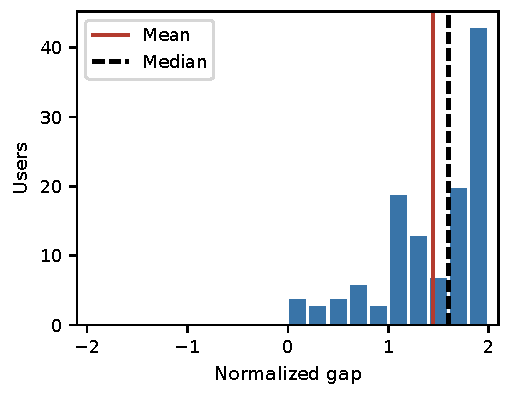
\includegraphics[width=\columnwidth]{docs/figures/observational_gap_distribution.pdf}
\caption{Distribution of the individual normalized gap among comparable users. Each user contributed equally to the primary mean.}
\label{fig:gap_support}\end{figure}

\begin{figure}[t]\centering
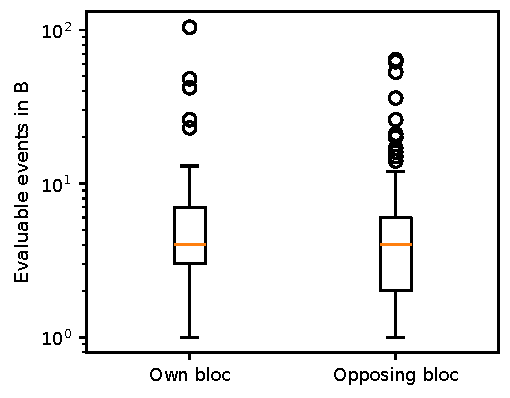
\includegraphics[width=\columnwidth]{docs/figures/observational_event_support.pdf}
\caption{Evaluable events per user in partition B, shown separately for the user's own bloc and the opposing bloc. The logarithmic scale preserved high-activity observations.}
\label{fig:event_support}\end{figure}

\begin{table*}[t]\centering\small
\caption{Summary statistics for comparable users.}
\label{tab:robustos}
\begin{tabular}{lrrrrr}\toprule
Metric & Mean & SD & Median & IQR & 10\% trimmed mean\\\midrule
AP$_{In}$ & 3.328 & 8.609 & 2.000 & [1.000, 4.000] & 2.541\\
AP$_{Out}$ & -6.090 & 9.600 & -3.000 & [-5.750, -2.000] & -4.000\\
AP & 9.418 & 14.296 & 6.000 & [4.000, 10.000] & 6.837\\
Dispersion & 2.010 & 1.156 & 1.789 & [1.414, 2.236] & 1.817\\
Normalized gap & 1.442 & 0.547 & 1.600 & [1.000, 2.000] & 1.511\\
\bottomrule\end{tabular}
\par\smallskip\footnotesize SD: standard deviation. IQR was reported as [25th, 75th percentile]. The trimmed mean removed 10\% of observations from each tail.
\end{table*}

High activity affected count-based balances more than the normalized primary contrast. Removing the right-affinity user with AP$_{In}=80$ reduced that group's mean AP$_{In}$ from 3.6481 to 2.2075, while the overall gap changed only from 1.4424 to 1.4410. Removing each user in turn left mean gaps between 1.4378 and 1.4543. Table~\ref{tab:robustos} summarized the skewed count distributions. The stability of the normalized gap under these exclusions showed that the primary finding did not depend on the most active user or on any single history.

\begin{figure}[t]\centering
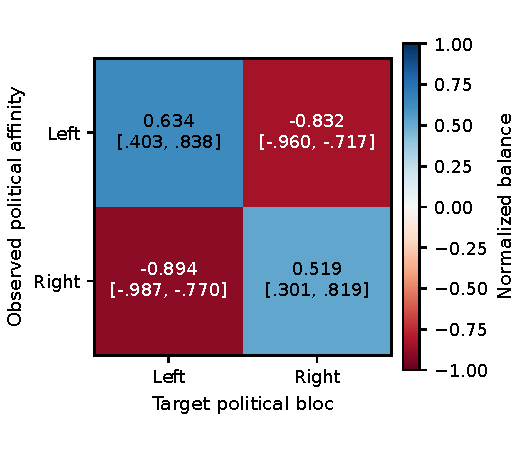
\includegraphics[width=\columnwidth]{docs/figures/observational_balance_matrix.pdf}
\caption{Normalized balances by observed affinity and target bloc, with 95\% CIs. Cells averaged users; positive values indicated net favorable evaluation.}
\label{fig:balance_matrix}\end{figure}

Figure~\ref{fig:balance_matrix} showed the political structure of the aggregate contrast: each affinity group had a favorable balance toward its own bloc and an unfavorable balance toward the other, with all four intervals retaining their signs. Support for aligned actors and rejection of opponents therefore coexisted in both groups, locating the observed differentiation in evaluations of competing political options. This pattern linked the measured gap to the study's electoral setting. It concerned political actors rather than hostility toward their supporters, and did not establish which affinity group was more polarized.

Figures~\ref{fig:ap_in} and~\ref{fig:ap_out} detailed the two components of that pattern. The presence of negative ingroup balances showed that observed affinity did not imply uniform approval: some participants expressed more unfavorable than favorable evaluations of their own bloc in B. This was evidence of internal criticism alongside political alignment, not an estimated change in voting preference; A and B were separate video sets rather than successive electoral periods. The predominantly negative outgroup balances showed the place of adversary-directed rejection in the discussion. Their extended negative tails represented accumulated unfavorable evaluations whose magnitudes also depended on participation. They did not establish stronger hostility or greater polarization in one affinity group.

Figure~\ref{fig:ap} combined these components into the count-based contrast. Its positive concentration showed how favorable differentiation accumulated across the observed histories, while large values could combine repeated participation with divergent evaluations of the two blocs. This distinction mattered politically: a prolific expression of opposition did not by itself indicate a stronger relative preference than that expressed by a less active participant. Reading this figure alongside the normalized gap in Figure~\ref{fig:gap_support} separated accumulated expression from the relative direction of evaluations.

Figure~\ref{fig:spread} summarized heterogeneity in balance magnitudes within each affinity group. The spread measure squared the balances and therefore discarded their signs; a high value alone did not identify support for aligned actors combined with rejection of opponents. Its political interpretation depended on the signed balances in Figures~\ref{fig:balance_matrix}--\ref{fig:ap_out}. The distributions showed that participants sharing an observed affinity did not express evaluations uniformly. Relative frequencies and common bin boundaries in Figures~\ref{fig:ap_in}--\ref{fig:spread} accommodated unequal group sizes. These figures provided complementary views of the same histories, rather than independent tests of polarization.

\begin{figure}[t]
\centering
\begin{tikzpicture}\begin{axis}[width=0.95\columnwidth,height=4.3cm,
xlabel={$\mathrm{AP}_{In}$},ylabel={Relative frequency},ymin=0,tick label style={font=\footnotesize},label style={font=\small},legend style={font=\footnotesize,at={(0.98,0.98)},anchor=north east},scaled ticks=false]
\addplot+[ybar interval,mark=none,fill opacity=0.25,draw=blue!70!black,fill=blue!70!black] coordinates {(-29,0.014705882) (-23.55,0) (-18.1,0) (-12.65,0) (-7.2,0) (-1.75,0.64705882) (3.7,0.27941176) (9.15,0.044117647) (14.6,0) (20.05,0) (25.5,0) (30.95,0.014705882) (36.4,0) (41.85,0) (47.3,0) (52.75,0) (58.2,0) (63.65,0) (69.1,0) (74.55,0) (80,0)};
\addplot+[ybar interval,mark=none,fill opacity=0.25,draw=orange!80!black,fill=orange!80!black] coordinates {(-29,0) (-23.55,0) (-18.1,0) (-12.65,0) (-7.2,0.055555556) (-1.75,0.66666667) (3.7,0.24074074) (9.15,0.018518519) (14.6,0) (20.05,0) (25.5,0) (30.95,0) (36.4,0) (41.85,0) (47.3,0) (52.75,0) (58.2,0) (63.65,0) (69.1,0) (74.55,0.018518519) (80,0)};
\legend{Left ($n=68$),Right ($n=54$)}
\end{axis}\end{tikzpicture}
\caption{Distribution of AP$_{In}$ by observed political affinity, using 20 common bins and relative frequencies within groups.}
\label{fig:ap_in}
\end{figure}

\begin{figure}[t]
\centering
\begin{tikzpicture}\begin{axis}[width=0.95\columnwidth,height=4.3cm,
xlabel={$\mathrm{AP}_{Out}$},ylabel={Relative frequency},ymin=0,tick label style={font=\footnotesize},label style={font=\small},legend style={font=\footnotesize,at={(0.98,0.98)},anchor=north east},scaled ticks=false]
\addplot+[ybar interval,mark=none,fill opacity=0.25,draw=blue!70!black,fill=blue!70!black] coordinates {(-62,0.029411765) (-58.9,0) (-55.8,0) (-52.7,0.014705882) (-49.6,0) (-46.5,0) (-43.4,0) (-40.3,0) (-37.2,0) (-34.1,0) (-31,0) (-27.9,0.014705882) (-24.8,0) (-21.7,0.014705882) (-18.6,0.014705882) (-15.5,0.058823529) (-12.4,0.058823529) (-9.3,0.058823529) (-6.2,0.26470588) (-3.1,0.47058824) (0,0)};
\addplot+[ybar interval,mark=none,fill opacity=0.25,draw=orange!80!black,fill=orange!80!black] coordinates {(-62,0) (-58.9,0) (-55.8,0) (-52.7,0) (-49.6,0) (-46.5,0) (-43.4,0) (-40.3,0) (-37.2,0) (-34.1,0) (-31,0.018518519) (-27.9,0) (-24.8,0) (-21.7,0.018518519) (-18.6,0) (-15.5,0) (-12.4,0.018518519) (-9.3,0.074074074) (-6.2,0.27777778) (-3.1,0.59259259) (0,0)};
\legend{Left ($n=68$),Right ($n=54$)}
\end{axis}\end{tikzpicture}
\caption{Distribution of AP$_{Out}$ by observed political affinity, using 20 common bins and relative frequencies within groups.}
\label{fig:ap_out}
\end{figure}

\begin{figure}[t]
\centering
\begin{tikzpicture}\begin{axis}[width=0.95\columnwidth,height=4.3cm,
xlabel={AP},ylabel={Relative frequency},ymin=0,tick label style={font=\footnotesize},label style={font=\small},legend style={font=\footnotesize,at={(0.98,0.98)},anchor=north east},scaled ticks=false]
\addplot+[ybar interval,mark=none,fill opacity=0.25,draw=blue!70!black,fill=blue!70!black] coordinates {(-1,0.30882353) (4.55,0.35294118) (10.1,0.19117647) (15.65,0.058823529) (21.2,0.044117647) (26.75,0.014705882) (32.3,0) (37.85,0) (43.4,0) (48.95,0) (54.5,0) (60.05,0) (65.6,0.014705882) (71.15,0) (76.7,0) (82.25,0) (87.8,0) (93.35,0.014705882) (98.9,0) (104.45,0) (110,0)};
\addplot+[ybar interval,mark=none,fill opacity=0.25,draw=orange!80!black,fill=orange!80!black] coordinates {(-1,0.38888889) (4.55,0.5) (10.1,0.074074074) (15.65,0.018518519) (21.2,0) (26.75,0) (32.3,0) (37.85,0) (43.4,0) (48.95,0) (54.5,0) (60.05,0) (65.6,0) (71.15,0) (76.7,0) (82.25,0) (87.8,0) (93.35,0) (98.9,0) (104.45,0.018518519) (110,0)};
\legend{Left ($n=68$),Right ($n=54$)}
\end{axis}\end{tikzpicture}
\caption{Distribution of AP by observed political affinity, using 20 common bins and relative frequencies within groups.}
\label{fig:ap}
\end{figure}

\begin{figure}[t]
\centering
\begin{tikzpicture}\begin{axis}[width=0.95\columnwidth,height=4.3cm,
xlabel={Dispersion},ylabel={Relative frequency},ymin=0,tick label style={font=\footnotesize},label style={font=\small},legend style={font=\footnotesize,at={(0.98,0.98)},anchor=north east},scaled ticks=false]
\addplot+[ybar interval,mark=none,fill opacity=0.25,draw=blue!70!black,fill=blue!70!black] coordinates {(0.40824829,0.044117647) (0.75436047,0.058823529) (1.1004726,0.11764706) (1.4465848,0.20588235) (1.792697,0.23529412) (2.1388092,0.058823529) (2.4849214,0.073529412) (2.8310335,0.11764706) (3.1771457,0) (3.5232579,0.014705882) (3.8693701,0.014705882) (4.2154823,0) (4.5615944,0.014705882) (4.9077066,0) (5.2538188,0) (5.599931,0.014705882) (5.9460432,0) (6.2921553,0) (6.6382675,0.014705882) (6.9843797,0.014705882) (7.3304919,0)};
\addplot+[ybar interval,mark=none,fill opacity=0.25,draw=orange!80!black,fill=orange!80!black] coordinates {(0.40824829,0) (0.75436047,0.18518519) (1.1004726,0.16666667) (1.4465848,0.24074074) (1.792697,0.2037037) (2.1388092,0.11111111) (2.4849214,0.037037037) (2.8310335,0) (3.1771457,0.018518519) (3.5232579,0) (3.8693701,0) (4.2154823,0.018518519) (4.5615944,0) (4.9077066,0) (5.2538188,0) (5.599931,0) (5.9460432,0) (6.2921553,0) (6.6382675,0) (6.9843797,0.018518519) (7.3304919,0)};
\legend{Left ($n=68$),Right ($n=54$)}
\end{axis}\end{tikzpicture}
\caption{Distribution of dispersion by observed political affinity, using 20 common bins and relative frequencies within groups.}
\label{fig:spread}
\end{figure}

\subsection{Robustness across specifications}
The aggregate direction survived changes in actor composition and contribution by video. All six intervals in Table~\ref{tab:sensibilidades} retained a positive gap. Balancing by video retained all 122 users; other variants reduced the sample. Paired changes against the original definition on the same retained users all included zero in their intervals. This convergence supported the direction of the aggregate finding across the examined specifications; it did not establish equivalence between their magnitudes.
\begin{table}[t]\centering\small
\caption{Original sensitivity variants and 95\% CIs.}
\label{tab:sensibilidades}
\setlength{\tabcolsep}{3pt}
\begin{tabular}{lrrr}\toprule
Variant & Users & Gap & 95\% CI\\\midrule
Reversed A/B & 76 & 1.520 & [1.227, 1.674]\\
Video-balanced & 122 & 1.473 & [1.284, 1.698]\\
Without Keiko Fujimori & 80 & 1.505 & [1.238, 1.709]\\
Without Roberto Sánchez & 90 & 1.447 & [1.294, 1.684]\\
Without Rafael López Aliaga & 98 & 1.506 & [1.318, 1.717]\\
Historical data only & 100 & 1.493 & [1.308, 1.755]\\
\bottomrule\end{tabular}\end{table}

Requiring more evidence per user reduced the observed sample without reversing the pattern. The fixed 12-combination grid retained 66--123 users, with gaps of 1.4306--1.5176 and entirely positive intervals. Requiring three events per bloc retained 66 users, gap 1.4059 [1.2032, 1.6715]; five per bloc retained 30, gap 1.3954 [1.0908, 1.6829]. These checks showed a tradeoff between individual support and breadth of observation. They were defined after the primary result and did not replace the main eligibility criteria.

Neutral evaluations moderated the normalized contrast. Removing them from denominators left 114 users with a gap of 1.6687 [1.5070, 1.8853], compared with 1.4827 under the original definition on those same users: change 0.1859 [0.0897, 0.2883]. Eight users lost valid denominators and received no imputed score. The primary definition retained neutral evidence; the alternative examined how its treatment changed magnitude. The supplement reported all specifications.

The pattern was also observable under neutral news sources, rather than being confined to explicitly aligned sources. Restricting B by editorial provenance yielded gaps of 1.4969 [1.1876, 1.7877] under left-wing sources ($n=63$), 1.3809 [0.7845, 1.9208] under right-wing sources ($n=16$), and 1.4676 [1.0788, 1.7772] under neutral sources ($n=52$). Users were required to retain both target blocs within each subset and could appear under several source groups. The smaller right-source sample had greater uncertainty. These conditional findings described settings of expression; they did not estimate channel effects.

\subsection{Individual stability and error sensitivity}
The A/B comparison did not establish that reusing affinity evidence necessarily inflated the observed contrast. Among 113 users measurable in both partitions, mean gaps were 1.5810 in A and 1.4152 in B; A minus B was 0.1658, 95\% CI [$-0.0494$, 0.3290]. The point estimate was compatible with optimism from reusing A, but the interval included zero. Separating evidence remained a design precaution rather than a conclusion derived from this test.

Individual rankings were substantially less stable than the aggregate direction. Across 200 B-video splits, 51--74 users were measurable in both halves (median 63). Median Pearson correlation was 0.3667, IQR [0.3032, 0.4203]; median Spearman correlation was 0.3806 [0.3272, 0.4448]. These IQRs described variation across partitions, not 95\% CIs. The scores characterized observed expressions, but their limited half-sample stability did not support treating each user as having a precisely measured, persistent psychological trait.

The aggregate direction remained positive under the examined adversarial error budgets of up to 10\%, conditional on fixed affinities, comparability, targets, and denominators. With affinities, comparability, targets, and denominators fixed, adversarially changing 80 of 1\,609 B events (5\% budget) left a minimum gap of 0.6391; 160 changes (10\%) left 0.1801; 321 changes (20\%) yielded $-0.5407$. The first nonpositive mean required 193 directed changes (12.00\%). This conditional bound examined the most influential B evaluations. It estimated neither actual annotation error nor errors in affinity, extraction, or selection, and did not validate a classifier.

\subsection{Classifier performance}
\begin{table*}[t]\centering\small
\caption{Targeted sentiment classification before abstention. Intervals used video bootstrap resampling; the panels retained different evaluation denominators.}
\label{tab:clasificadores}
\begin{tabular}{lrrrr}\toprule
& \multicolumn{2}{c}{End-to-end evaluation} & \multicolumn{2}{c}{Common complete context}\\
Model & Macro-F1 & 95\% CI & Macro-F1 & 95\% CI\\\midrule
RoBERTuito & 0.3836 & [0.3578, 0.4118] & 0.5979 & [0.5771, 0.6174]\\
BETO & 0.3237 & [0.3014, 0.3477] & 0.4993 & [0.4814, 0.5173]\\
XLM-RoBERTa & 0.2832 & [0.2620, 0.3059] & 0.4309 & [0.4143, 0.4477]\\
MrBERT-es & 0.3225 & [0.3010, 0.3460] & 0.5025 & [0.4838, 0.5202]\\
mDeBERTa-v3-base & 0.3086 & [0.2871, 0.3320] & 0.4733 & [0.4564, 0.4905]\\
\bottomrule\end{tabular}\end{table*}

Table~\ref{tab:clasificadores} compared five models on 5\,165 annotation--prediction pairs in the end-to-end evaluation and 3\,222 shared complete-context candidates. End-to-end scores included extraction omissions, whereas the common panel isolated classification on available inputs. RoBERTuito had the highest end-to-end macro-F1 (0.3836). The larger scores on complete-context inputs showed why classifier performance and the ability to recover all political targets had to be distinguished.
RoBERTuito exceeded each alternative in end-to-end macro-F1 under video-bootstrap contrasts with Holm adjustment. The two additional pretrained bases did not improve on that reference in this sample.
The comparison detected no clear difference between BETO and MrBERT-es; this did not establish equivalence. Model differences combined architecture, pretraining, and tokenization rather than identifying a causal effect of any one component.
Accepted predictions covered 3.2--21.2\% of evaluable target weight across models, limiting automatic expansion; the supplement reported model-specific coverage, accepted precision, and extraction and abstention diagnostics. The polarization estimates came from annotated user histories and retained their own users and denominators; classifier outputs were not assigned to the full comment collection.

\subsection{Interpretation in Peru's 2026 election}
The results identified a consistent pattern of expressed affective polarization among the comparable users: political affinity differentiated favorable evaluations of aligned actors from unfavorable evaluations of opponents. This distinction gave substantive meaning to the positive normalized gap. The affinity--target matrix showed whom participants supported and rejected, while the distribution across users and the sensitivity analyses established that the aggregate direction was not confined to a few extreme histories or a single prominent actor.

This direction agreed with the positive ingroup balances and predominantly negative outgroup evaluations reported by Martínez-España et al. \cite{polariz}. The present study extended that measurement approach to YouTube electoral comments by distinguishing channel provenance, evaluated actors, and observed affinity, and by evaluating expressions in videos separate from those used to assign affinity. Normalization and sensitivity analyses addressed the influence of activity and actor composition on the aggregate contrast. Different group definitions, denominators, and sampling rules precluded a numerical ranking of polarization across the two studies.

The findings also complemented earlier evidence from Peru. Ponte Torrel \cite{Ponte2022} documented emotionally differentiated support and rejection toward the rival presidential candidacies in Twitter discussions of the 2021 election. The present analysis added a within-user contrast between evaluations of aligned and opposing blocs in another platform and electoral period. This comparison linked the observed pattern to an established concern in Peruvian electoral communication, also situated within the longer political conflict discussed by Mejía Navarrete \cite{Mejia2024}; it did not estimate change between elections.

The electoral context provided a concrete setting for this interpretation. The JNE documented a runoff between Fuerza Popular and Juntos por el Perú after the April election \cite{JNE11352026}. The Defensoría del Pueblo recorded rejection of candidacies and opposing demands concerning the electoral process, describing polarized political confrontations \cite{Defensoria2842026}. The directed support and rejection observed on YouTube were consistent with this documented context of electoral antagonism. The institutional report supplied contextual evidence, while the present study characterized evaluations in the observed digital discussion. Because January--June comments were pooled, the analysis did not attribute the gap to particular events or estimate its evolution during the runoff.

The persistence of the contrast under neutral news sources further located these expressions within general news discussions. Political differentiation was observable even where channel provenance did not assign the discussion to either political bloc. Moreover, users with evaluable comments about both blocs still expressed relative favoritism, showing that evidence concerning opposing actors could coexist with affective differentiation. This finding concerned expressed evaluations; commenting about an actor did not establish direct interaction with that actor's supporters or an effect of the hosting channel.

The value of identifying the evaluated target also connected this study to the aspect-based analysis of YouTube comments by Miehling et al. \cite{Miehling2025}. Target-specific analysis distinguished evaluations that a single comment-level sentiment label could combine, consistent with the distinction between sentiment and political stance \cite{BestvaterMonroe2023}. Here, that distinction enabled an explicit comparison between aligned and opposing actors. Together, the results supported an aggregate interpretation of expressed affective polarization within the observed users, while the inconclusive affinity-group contrast and limited individual stability defined the level at which that interpretation was supported.

\section{Limitations}

This study examined expressed evaluations among active YouTube participants with evidence toward both political blocs. Its scope was defined by the selected channels, explicit mentions, and actors with documented bloc assignments (22 of 124 identities). The findings therefore characterized this observed discussion; population-level estimates for the Peruvian electorate were outside the sampling design.

Video partitions A and B separated affinity assignment from evaluation, while expressions by the same author remained related. The normalized gap reduced dependence on activity and was interpreted as an aggregate contrast. The split-half results called for caution when interpreting individual scores as persistent attributes.

The cohort was capped at 300 examined users for resource reasons after annotation progress was known, replacing the initial target of 800 comparable users. The observed confidence intervals were used to assess the precision achieved by this sample \cite{lakens2022sample}. Additional models and complementary checks were chosen after initial results had been examined, so their findings were interpreted as comparisons within this sample. Full sampling and diagnostic details were reported in the supplement.

\section{Conclusions and Future Work}
The study identified a consistent pattern of expressed affective polarization among 122 comparable YouTube users during Peru's 2026 electoral period. Favorable evaluations of aligned political actors coexisted with unfavorable evaluations of opposing actors, yielding a mean normalized gap of 1.44 (95\% CI [1.27, 1.68]). A positive gap occurred in 120 of the 122 users, showing that relative favoritism was broadly shared within this observed group. The central empirical contribution was the identification of the political direction of support and rejection within users' comment histories.

The positive aggregate direction persisted under actor exclusions, video balancing, and stricter evidence requirements, supporting the finding across the examined alternatives. Its presence under neutral news sources showed that affective differentiation also appeared in general news discussions. These findings complemented earlier evidence of candidate-directed affect in Peruvian electoral communication and were consistent with the documented context of electoral confrontation. The observed internal criticism also showed that alignment did not entail uniform approval of actors from the same bloc. Together, these findings characterized an electoral discussion in which differentiation between political options coexisted with diversity of evaluations within each affinity group.

The methodological contribution separated the source hosting a comment, the actor evaluated, and the author's observed affinity. Disjoint video sets separated affinity assignment from evaluation, while normalized balances and equal user weighting distinguished relative evaluation from the volume of participation. This design provided a reproducible way to examine directed political evaluations with explicit checks of sensitivity and measurement support. The complementary comparison of five classifiers identified RoBERTuito as the strongest evaluated model in end-to-end macro-F1 and distinguished target-recovery losses from classification performance. The user-history findings remained grounded in their annotations rather than extrapolated classifier predictions.

The conclusions concerned aggregate expressions among the studied users; persistent individual attributes and differences between affinity groups required further evidence. Future research priorities included broader target coverage, more evidence per user, improved resolution of ambiguous references, and comparisons across electoral periods. Within its observed scope, the study established a measurable pattern of support for aligned actors and rejection of opponents, and clarified how that pattern could be examined separately from general comment sentiment and channel orientation.


% \section{Conclusiones y trabajo futuro}

% En este trabajo se aplicó un enfoque simplificado, inspirado en la metodología de
% Martínez-España et al. \cite{polariz}, para analizar el sentimiento político
% expresado en comentarios de TikTok durante la segunda vuelta de las elecciones
% presidenciales peruanas de 2026, utilizando el modelo RoBERTuito sobre un conjunto
% de 2743 comentarios.

% Los resultados evidenciaron un comportamiento consistente con un \textit{echo
% chamber}: las publicaciones asociadas a ambos candidatos registraron favorabilidad
% neta positiva y de magnitud muy similar entre sí, en contraste con el clima
% levemente negativo de las publicaciones neutrales. Esta similitud entre bloques
% políticos, sumada al hecho de que el resultado electoral fue sumamente cerrado,
% refuerza la idea de que el sentimiento expresado en redes sociales debe entenderse
% como un reflejo del clima emocional de la conversación digital, y no como un
% predictor directo de la intención de voto.

% La principal limitación del estudio fue la escasa recurrencia de los usuarios: la
% gran mayoría comentó una única vez y prácticamente ninguno interactuó con
% publicaciones de más de una categoría política. Esto impidió calcular un indicador
% de polarización afectiva individual (\textit{ingroup}/\textit{outgroup}) equivalente
% al de la metodología de referencia \cite{polariz}, restringiendo los resultados a
% una medida de favorabilidad agregada por categoría.

% Como trabajo futuro se plantea ampliar el volumen y la diversidad de las fuentes de
% datos para captar usuarios recurrentes entre distintas orientaciones políticas,
% explorar la detección de menciones a otros candidatos dentro de un mismo comentario
% como señal adicional de polarización, e incorporar una validación manual del modelo
% de clasificación que permita cuantificar su desempeño sobre el dominio específico de
% comentarios políticos en español peruano.

% % conference papers do not normally have an appendix


% % use section* for acknowledgement
% % \section*{Acknowledgment}


% % The authors would like to thank...





% % trigger a \newpage just before the given reference
% % number - used to balance the columns on the last page
% % adjust value as needed - may need to be readjusted if
% % the document is modified later
% %\IEEEtriggeratref{8}
% % The "triggered" command can be changed if desired:
% %\IEEEtriggercmd{\enlargethispage{-5in}}

% % references section

% % can use a bibliography generated by BibTeX as a .bbl file
% % BibTeX documentation can be easily obtained at:
% % http://www.ctan.org/tex-archive/biblio/bibtex/contrib/doc/
% % The IEEEtran BibTeX style support page is at:
% % http://www.michaelshell.org/tex/ieeetran/bibtex/
% %\bibliographystyle{IEEEtran}
% % argument is your BibTeX string definitions and bibliography database(s)
% %\bibliography{IEEEabrv,../bib/paper}
% %
% % <OR> manually copy in the resultant .bbl file
% % set second argument of \begin to the number of references
% % (used to reserve space for the reference number labels box)

\bibliographystyle{IEEEtran}
\bibliography{IEEEabrv,docs/references}


\end{document}

